\subsection{Problem statements}
\begin{frame}{Background}
    RKB effectiveness for group collaboration
\begin{itemize}
    \item Some research works related to RKB \cite{Wunnasri2018ReciprocalUnderstanding,Wunnasri2018ReciprocalCollaboration}
    have focused on the RKB effect as preparation for collaboration
    \item They evaluated the learners' discussion and similarity of
    knowledge after following the activities
    \item Students do not need to integrate different understanding, after 
    discussion 
    \item In a practical situation, a joint outcome is expected
    \item To understand whether the collaborative activity has good performance
    \item By making a single product, students has to negotiate different understanding
\end{itemize}
\end{frame}

\subsection{Research objectives}
\begin{frame}{Research objectives}

\begin{block}{Aim}
    The focus of this particular study is to identify the effectiveness
    of approach for creating a collaborative product.
    % Does the RKB approach affect co-construction of knowledge with concept maps? 
    %If so, to what extent?
\end{block}

\begin{alertblock}{Sub-research questions}
    \begin{enumerate}
        % \item What is the score of group maps? % descriptive RQs
        % \item What is the score of individual maps?
        \item Is there a significant different between the learning outcomes as a group
        or as an individual?
        \item How is the pattern of map changes from individual to group?
        \item How is the affective response of the students while following the activities?
\end{enumerate}
\end{alertblock}

%% The study focuses on identifying the effectiveness from the end-products 
%% (collaborative maps), the patterns of map changes from individuals to groups, 
%% and the perceptions of the students while following the learning activities. 
\end{frame}

\subsection{Analysis methods}

\begin{frame}{Data measurements}
    \begin{alertblock}{Sub-research questions}
        \begin{itemize}
        \item Is there a significant different between the learning outcomes as a group
        or as an individual?
        \begin{itemize}
            \item evaluation of individual and group concept map by the teacher 
                  as a domain expert
            \item
        \end{itemize}
        
        \item How is the pattern of map changes from individual to group?
        \begin{itemize}
            \item a propositional-level similarity analysis
            \item
        \end{itemize}
        
        \item How is the affective response of the students while following the activities?
        \begin{itemize}
            \item conduct a survey on learners' experiences during each phase of RKB activities
            \item
        \end{itemize}
        \end{itemize}
    \end{alertblock}
\end{frame}
    %\begin{enumerate}
    %    \item Concept map scoring by an expert
    %    \item Proposition similarity
    %    \item Questionnaire on learner's affective response
    %\end{enumerate}

\begin{frame}{Concept map scoring}
    \begin{itemize}
        \item The teacher developed a grading rubric to evaluate students’ 
        concept maps that used the expert’s map as a criterion map 
        (Osmundson, Chung, Herl, \& Klein, 1999). 
        \item The teacher categorized the types of information that should be included in the map.
        \item \textcolor{red}{[@todo: add experts map, experts rubric]}
    \end{itemize}
\end{frame}

\begin{frame}{Proposition similarity}

\end{frame}

\begin{frame}{Questionnaire on learner's affective response}
    \begin{itemize}
        \item The survey covered items regarding the perspectives of 
              the students on the task itself (e.g., attractiveness 
              and stimulation scales) and the system used (or non-task; 
              e.g., perspicuity scale). 
        \item The questionnaire scales were adopted from the User Experience
              Questionnaire, an Indonesian version (Laugwitz, Held, \& Schrepp, 2008;
              Santoso, Schrepp, Kartono, Yudha, \& Priyogi, 2016). 
        \item The six open-ended questions were given to uncover the positive and
              negative experiences of the students during the experiment.
        \item \textcolor{red}{[@todo: add the sample of questions]}
    \end{itemize}
\end{frame}

\subsection{Results \& discussions}
\begin{frame}[allowframebreaks]{Results (1): Overall group performance}
\begin{table}[tb]
    \caption{Descriptive statistics}
    \label{a1::group_performance}
    \begin{center}
        \begin{tabular}{c|c|c}
            \hline
            & Individual-map score & Group-map score\\
            \hline
            $M$ & 72.21 & 90 \\
            $SD$ & 18.22 & 7.31 \\
            $Min.$ & 41.43 & 75.71 \\
            $Max.$ & 98.57 & 100 \\
            \hline
        \end{tabular}
    \end{center}
\end{table}

\begin{figure}[tb]
    \begin{center}
        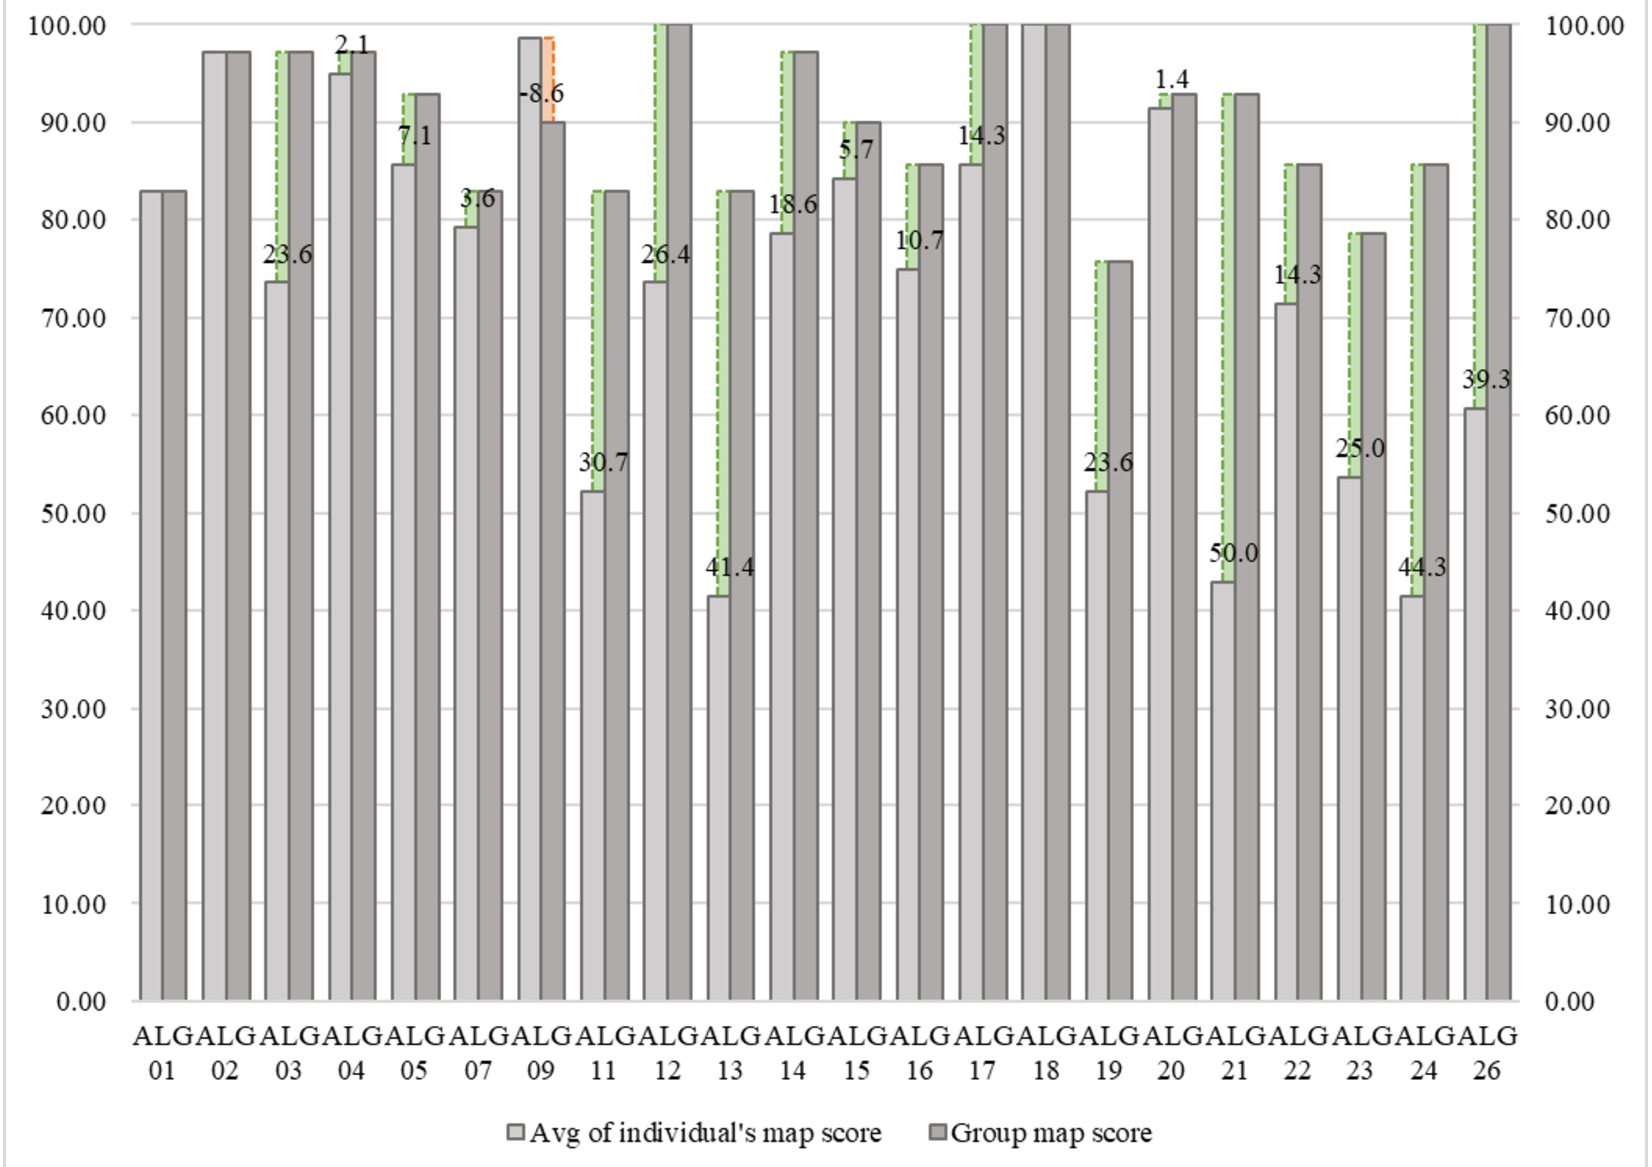
\includegraphics[width=80mm]{images/a1_mapscore_distribution.pdf}
    \end{center}
    \caption{Scores from the average of individual and group maps, along with the differences between the two scores}
    \label{a1::mapscore_distribution}
\end{figure}

\begin{table}[tb]
    \caption{Distribution of correctness level in all individual and group propositions}
    \label{dist_correct}
    \begin{center}
        \begin{tabular}{c|c|c}
            \hline
            Level of correctness & Individual-map (\%) & Group-map (\%)\\
            \hline
            The true proposition & 64 & 81 \\
            The false proposition with a minor error & 5 & 7 \\
            The false proposition with a moderate error & 10 & 7 \\
            The false proposition with a fatal error & 21 & 5 \\
            \hline
        \end{tabular}
    \end{center}
\end{table}

\begin{figure}[tb]
    \begin{center}
        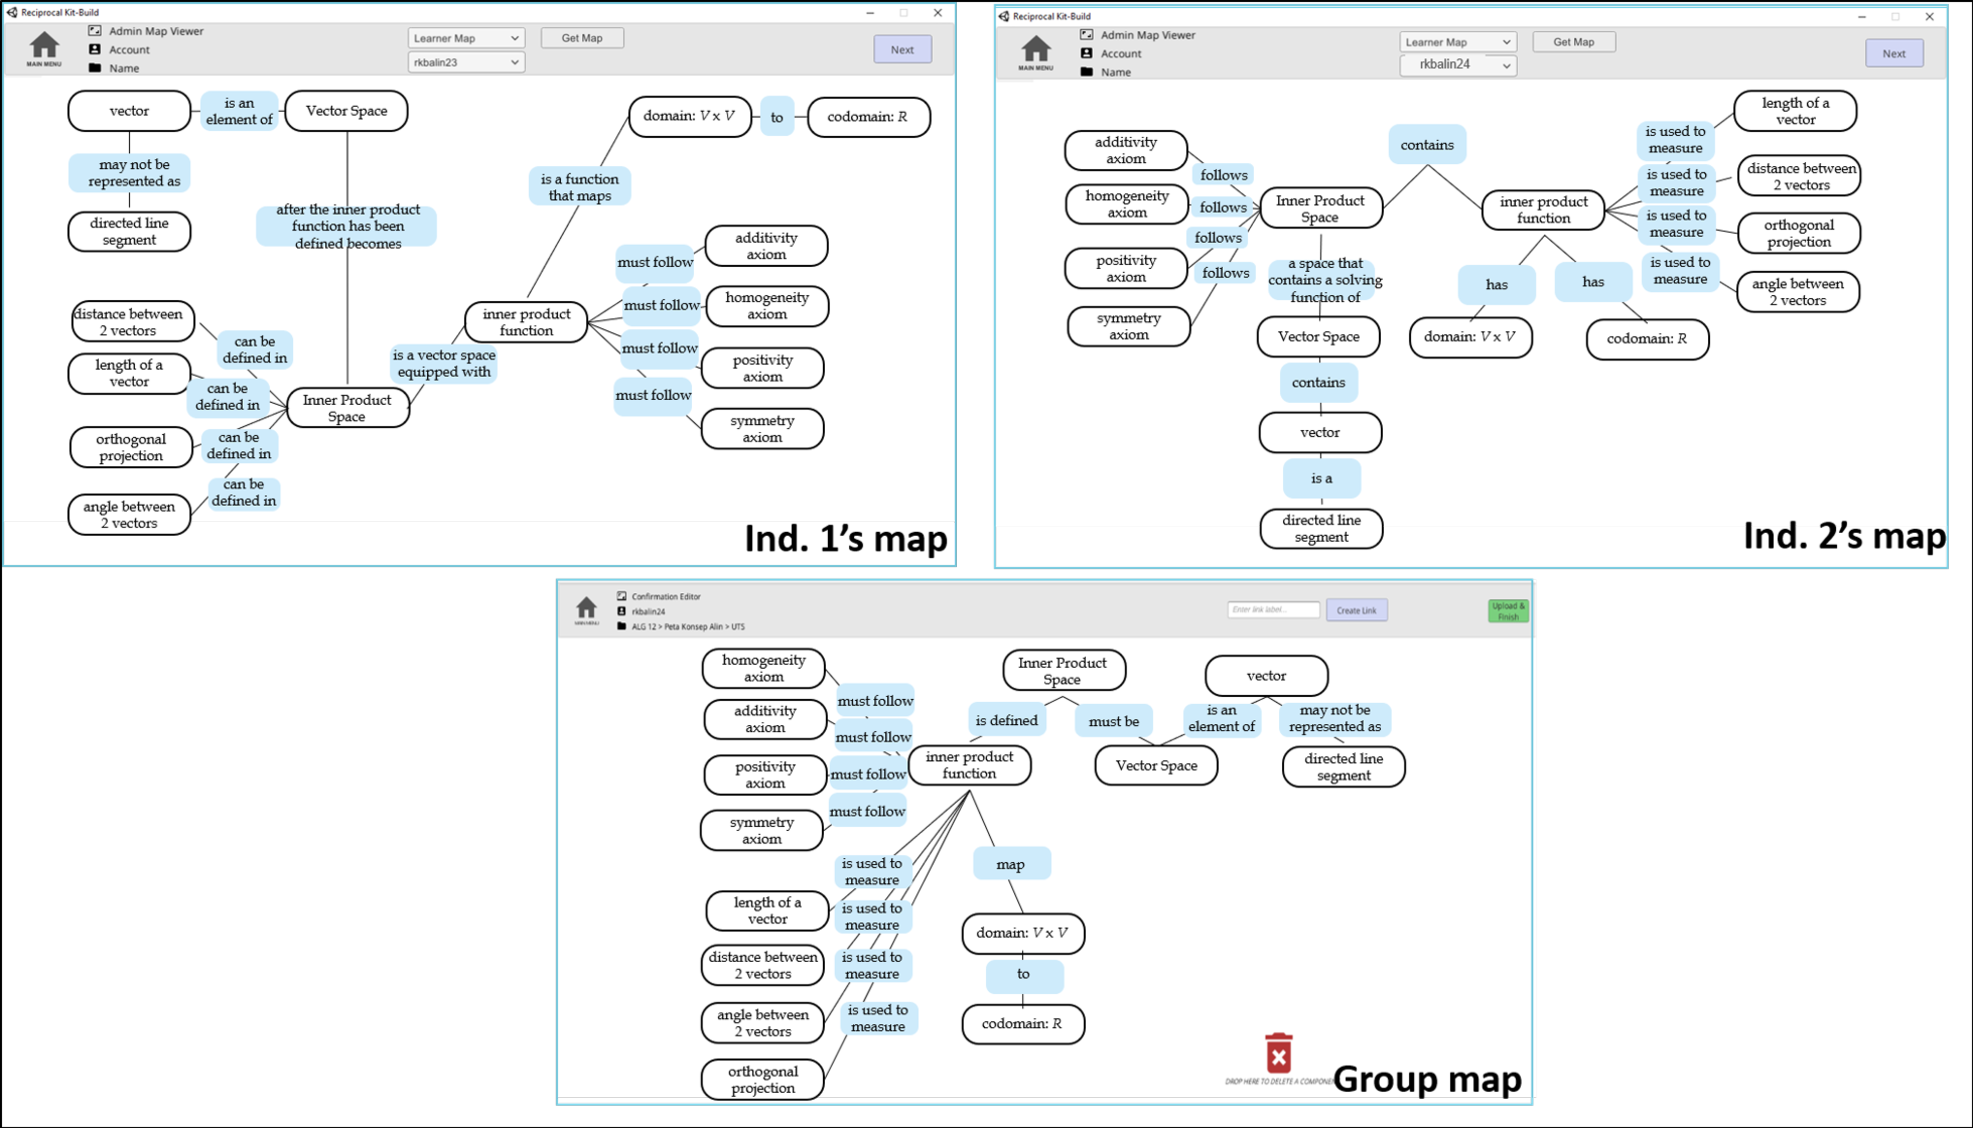
\includegraphics[width=100mm]{images/a1_dist_correctness.pdf}
    \end{center}
    \caption{Sample of individual maps and group map generated by group ALG12}
    \label{a1::map_sample}
\end{figure}

\end{frame}

\subsection{Implications of findings}